\documentclass[12pt,letterpaper]{article}

\title{Honors Thesis Poster}

\usepackage{hyperref}
\usepackage{setspace}
\usepackage{amsmath}%
\usepackage{MnSymbol}%
\usepackage{wasysym}%
\usepackage{lmodern}


\usepackage[utf8]{inputenc}
\usepackage[T1]{fontenc}
\usepackage[sfdefault,lf]{carlito}

\usepackage[margin=1.1cm,letterpaper]{geometry}
\usepackage{multicol}
\usepackage{ragged2e}
\usepackage{tabularx}
\usepackage[table]{xcolor}
\usepackage{graphicx}

\definecolor{OverleafGreen}{HTML}{4F9C45}
\graphicspath{{img/}}
\pagestyle{empty}
\RaggedRight
\parskip=12pt plus 4pt

\begin{document}


{\fontsize{40pt}{42pt}\bfseries\selectfont\color{OverleafGreen}%
Evolvability: What Is It and How Do We Get It?%
} \hfill {\LARGE\bfseries%
\mbox{4pm, Wed March 22, Th 391}%
}

\vspace{-2ex}


\begin{large}
\justify
{\setstretch{0.9} Biological organisms exhibit spectacular adaptation to their environments. However, another marvel of biology lurks behind the adaptive traits that organisms exhibit over the course of their lifespans: it is hypothesized that biological organisms also exhibit adaptation to the evolutionary process itself. That is, biological organisms are thought to possess traits that facilitate evolution. The term evolvability was coined to describe this type of adaptation. The question of evolvability has special practical relevance to computer science researchers engaged in longstanding efforts to harness evolution as an algorithm for automated design. It is hoped that a more nuanced understanding of biological evolution will translate to more powerful digital evolution techniques. This talk will present a theoretical overview of evolvability, illustrated with examples from biology and evolutionary computing, and discuss computational experiments probing the relationship between environmental influence on the phenotype and evolvability.\par}

\end{large}

{\LARGE\bfseries An Honors Thesis Presentation \hfill $\blacksquare$ \hfill Light Refreshments Served}\par%

{\centering%
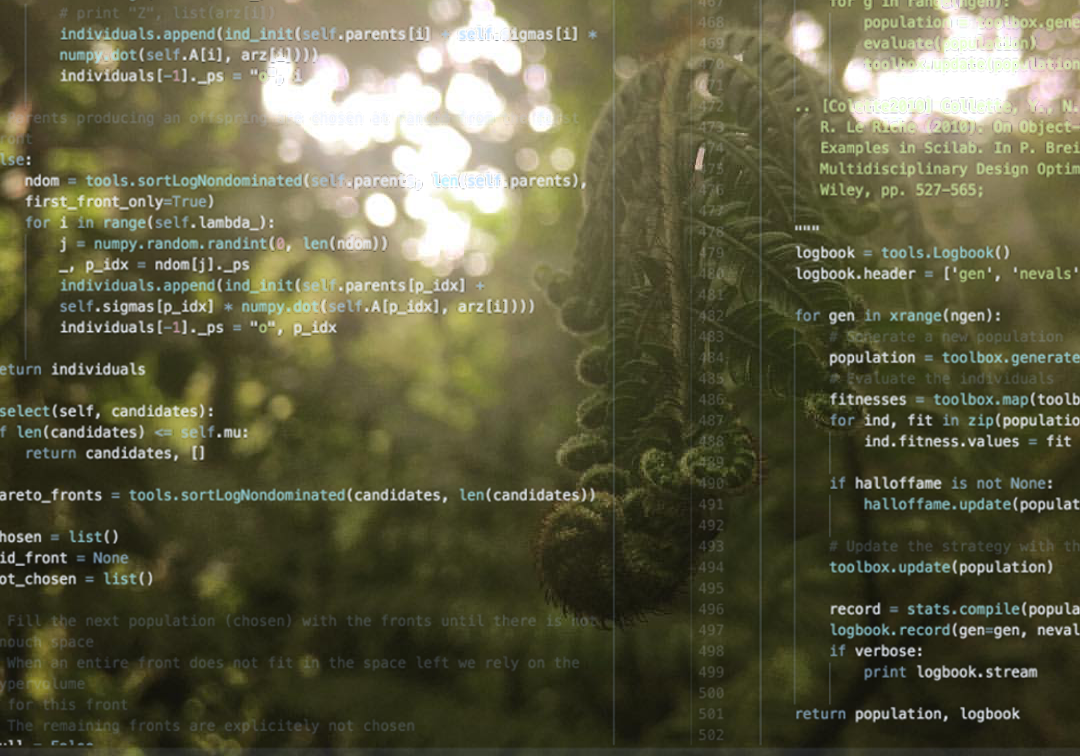
\includegraphics[width=\linewidth]{postergraphic_cropped}%
\par}

\vfill

{\LARGE Matthew Moreno}
\hfill
{\Large \url{https://mmore500.github.io}}
\end{document}